\documentclass[../Main.tex]{subfiles}
\begin{document}


This section describes functionality and design principles of implemented mobile application for 
style transfer. We will present whole application screen by screen and some
of the difficulties we were facing during development.

\subsection{Requirements}
During planning process we decided that our application should meet all of the 
below requirements.
User should be able to:
\begin{itemize}
    \item manage filters in some kind of gallery, where it's easy to pick filter image
    \item take photo directly in application and then use it as filter
    \item set style transfer settings like color preservation or scale
    \item transfer style from filter to real-time video
\end{itemize}

\subsection{Design}
Our assumption was to fill our application with beautiful image content,
painters greatest pieces of work so every user should feel like he's communing with art.
To achieve this goal we let images take whole screen and put them on first plane.
Most of the UI elements are transparent in some level so they don't cover the images.
Buttons and icons are very subtle, kept in Google's Material Design style.
Animations are also gentle and they are introduced to improve user experience rather
than make mind blowing visual effects.

\subsection{Difficulties}
To create style transfer client application and meet all of the requirements
we had to face two main difficulties:
\begin{itemize}
    \item sending video to server and than receiving it back with applied style transfer (real-time streaming)
    \item implementing efficient image gallery which can load photos from smartphone's storage
\end{itemize}

Our main concept of this project was real-time streaming so solving first problem was crucial.
A great, relatively new tool for streaming video is WebRTC.
It's HTML5 standard and it allows real-time communication in browser. 
Someone may wonder how this can allow us to stream video in mobile application.
We used Flutter InAppWebView plugin which can display websites inside application.
With this plugin we were able to move almost all logic associated with communication into server.
The application is just opening website under hardcoded specific address.

The second task was to create effective custom image gallery. 
Most smartphones take high resolution pictures which size is around 3-4 MB.
It takes long time for Flutter to load big pictures like these especially when
we have to load twelve or even more. We needed to load loads of pictures but they could be in fact very small because they ought to be presented as the thumbnails.
In addition to there is problem with 
memory overflow - when we were loading all picture at once application was
crashing after few second. 
To face memory overflow and high loading times introduced two improvements:
lazy loading and image resize in line with compression.
The gallery loads only twelve pictures at time so memory won't be filled so quickly.
Improved gallery is also resizing file to $400\times400$ resolution and then compression is applied.
It let us to save us memory and time.


\subsection{Application walk-through}
This part presents final client aplication and all it's capabilities.
Every screenshot comes from Huawei P10 Lite with Android 8.1 operating system. In the pictures we can see aplication design which was desribed in chapter 0.2.

\subsubsection{Start screen}
Star screen appears just after aplication is loaded. It has only aesthetic purpose and it's introduction to main part of aplication. We can see here Vincent van Gogh picture \textit{Seascape near Les Saintes-Maries-de-la-Mer} and it's just one of 27 pre-built image-filters. Screen contains also aplication name \textit{ARTEXTURE}. If we would like to go to next screen we have to swipe up or tap arrow button on the botom.


\begin{figure}[H]
    \centering
    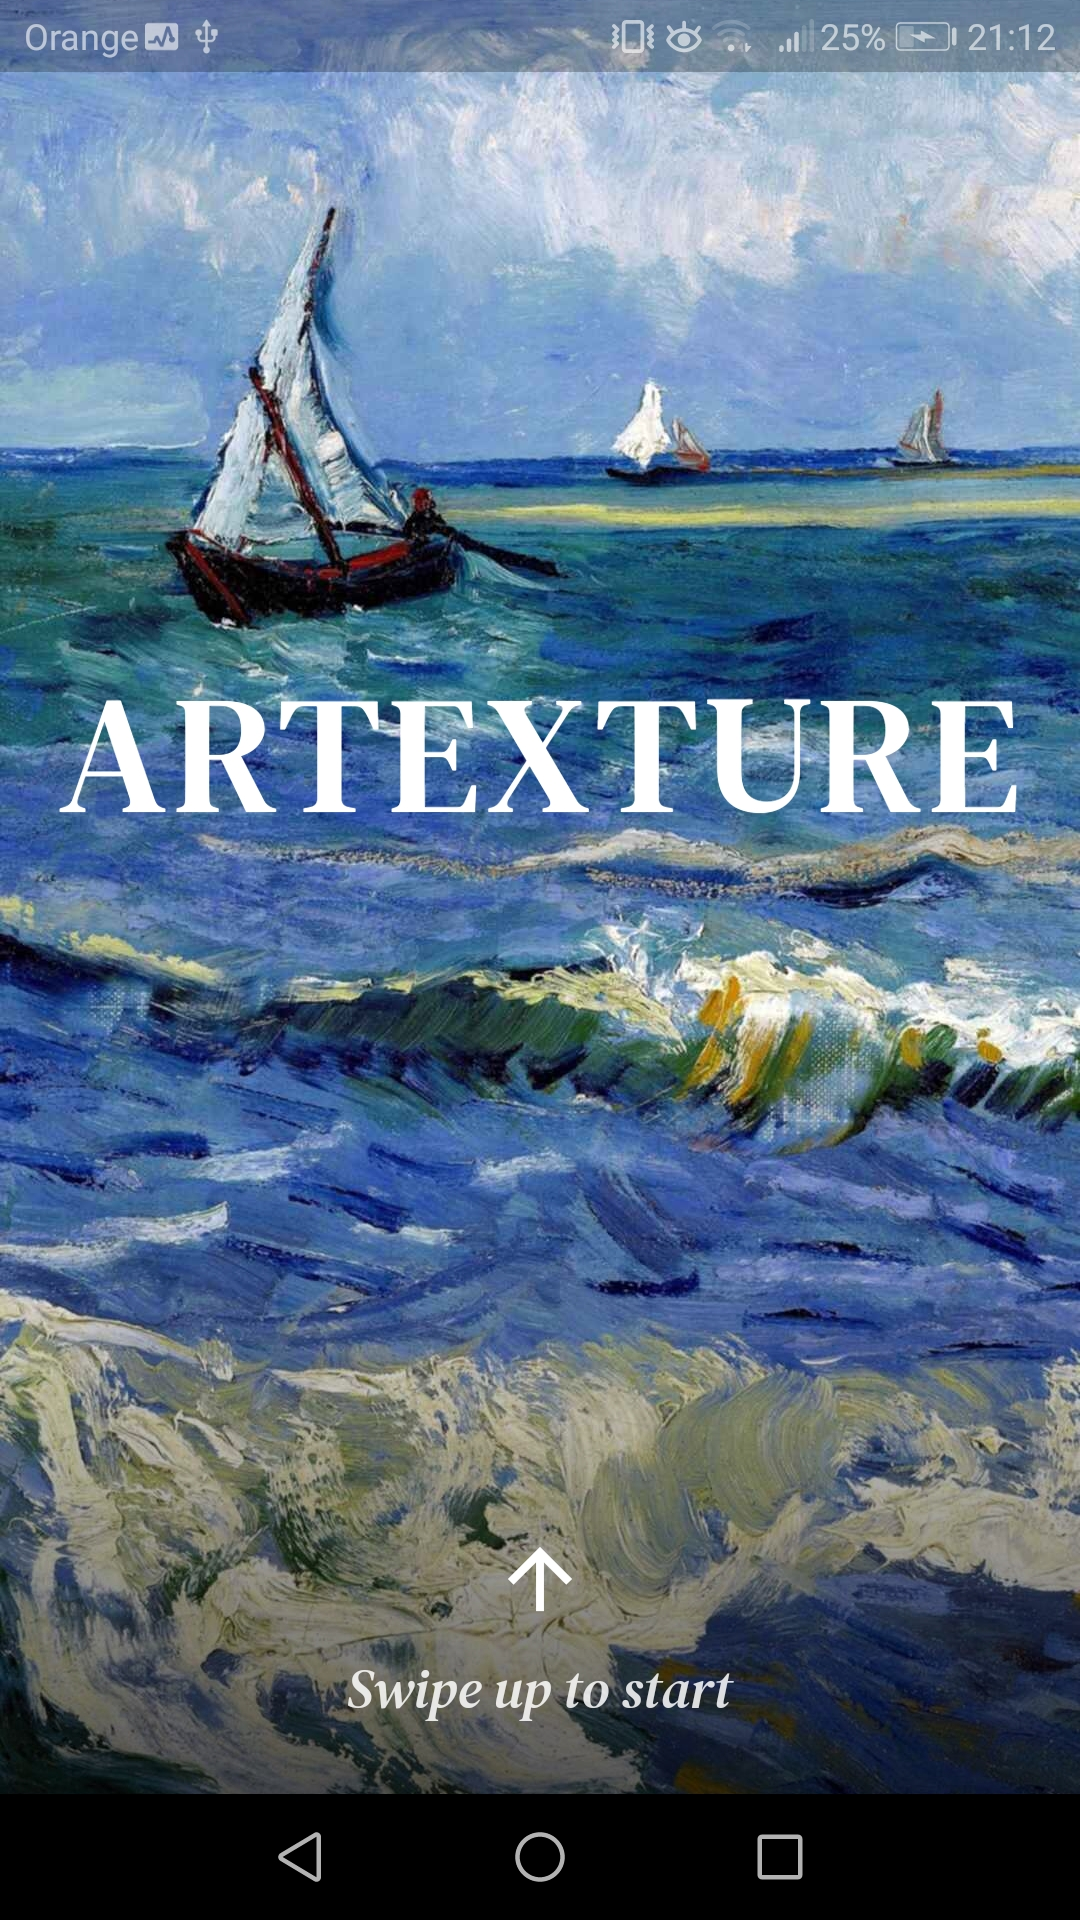
\includegraphics[width=0.325\textwidth]{start_screen.jpg}
    \caption{Start screen}
    \label{fig:start-screen}
\end{figure}


\subsubsection{Gallery}
Gallery is a main screen of the application. It allows us to pick image 
which we want to use as a filter. Bottom half of the screen is taken by list of images and it is presented at Figure \ref{fig:gallery_unfolded}.
Application comes with 27 built in paintings images. We can also use images from storage.
To switch between this two you have to click pallet icon on image icon on top of the list.
If we select one of images from list it appears immediately in the background.
In order to have a good look on whole selected image there is a possibility 
to hide list by clicking on down arrow icon (Figure \ref{fig:gallery_folded}).
In right upper corner there is settings icon and after tapping we can see a 
alert box (Figure \ref{fig:gallery_options}) with two filter settings:
\textit{intensity} and \textit{color preservation}.
Next to settings icon there is a plus icon which lead us \textit{Pick a filter} 
screen described later.

\begin{figure}[H]
    \minipage{0.32\textwidth}
        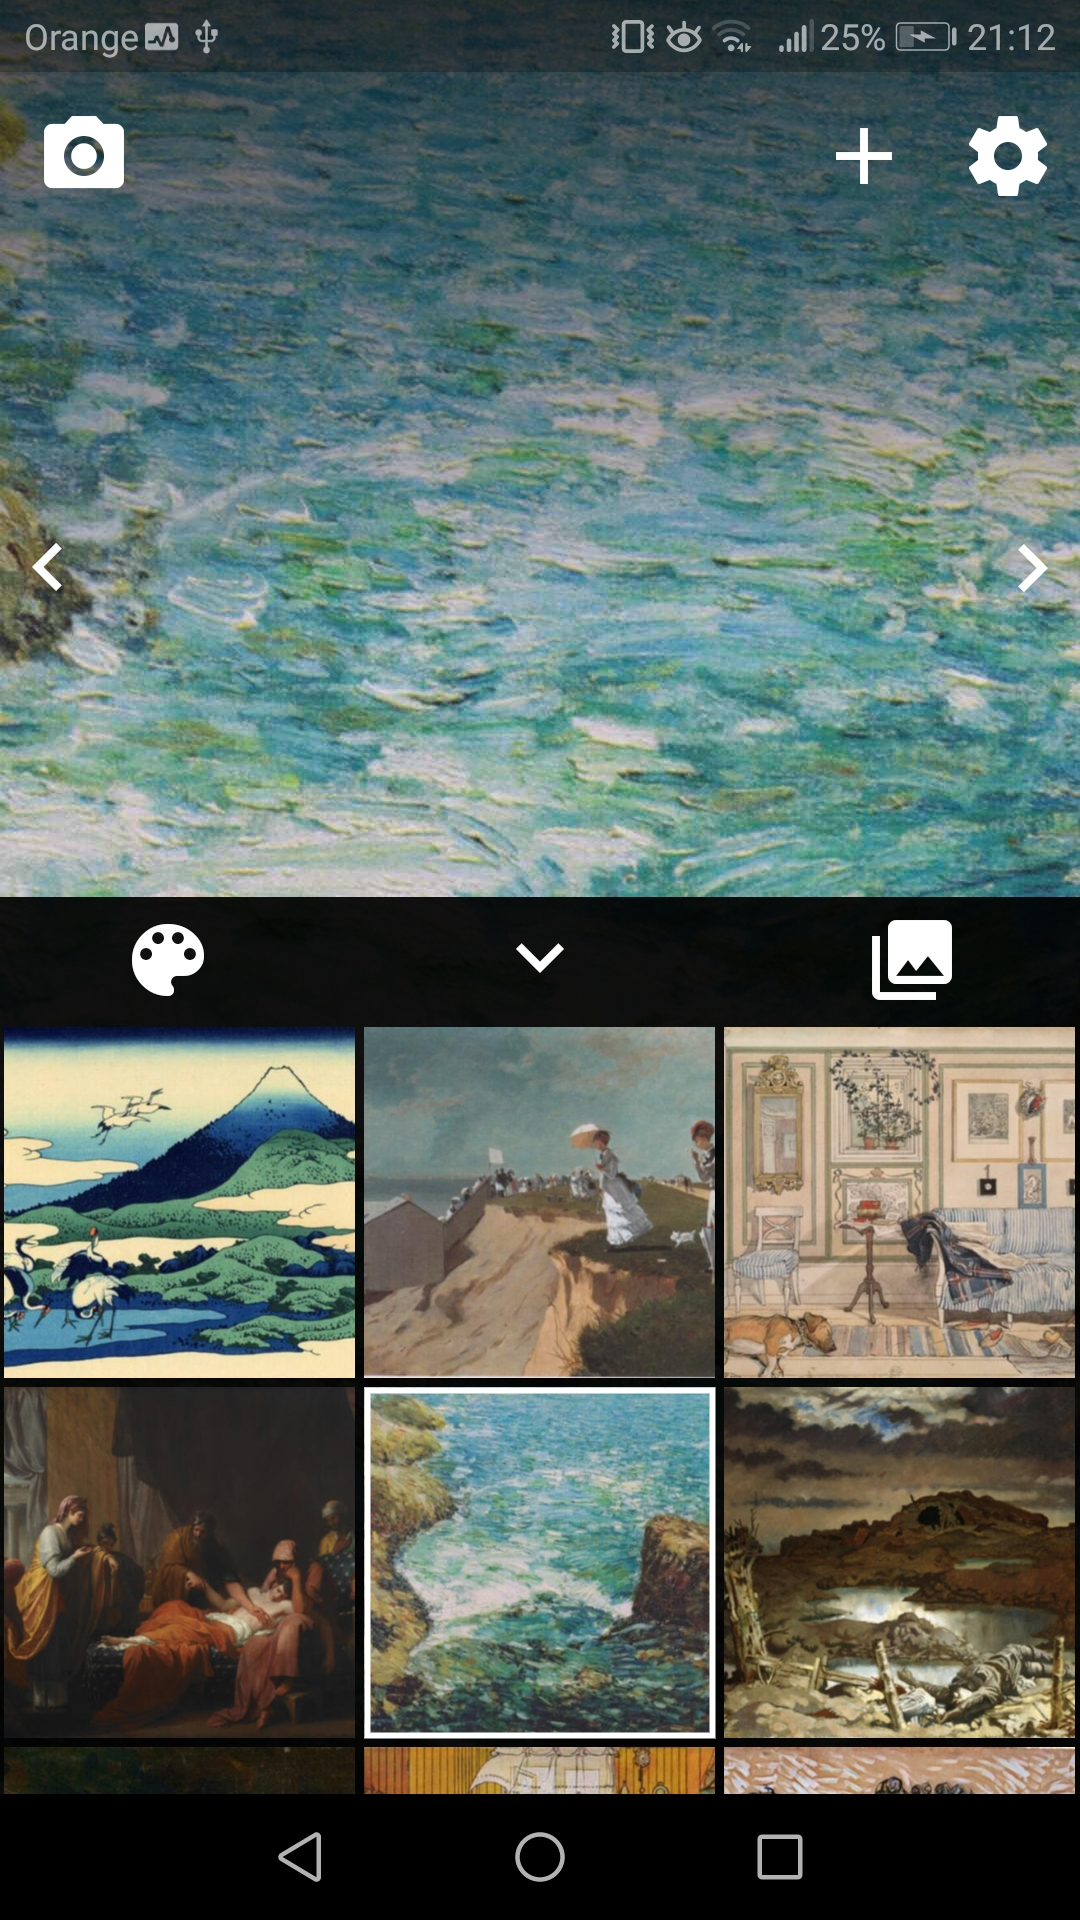
\includegraphics[width=\linewidth]{gallery_1.jpg}
        \caption{Unfolded gallery}\label{fig:gallery_unfolded}
    \endminipage\hfill
    \minipage{0.32\textwidth}
        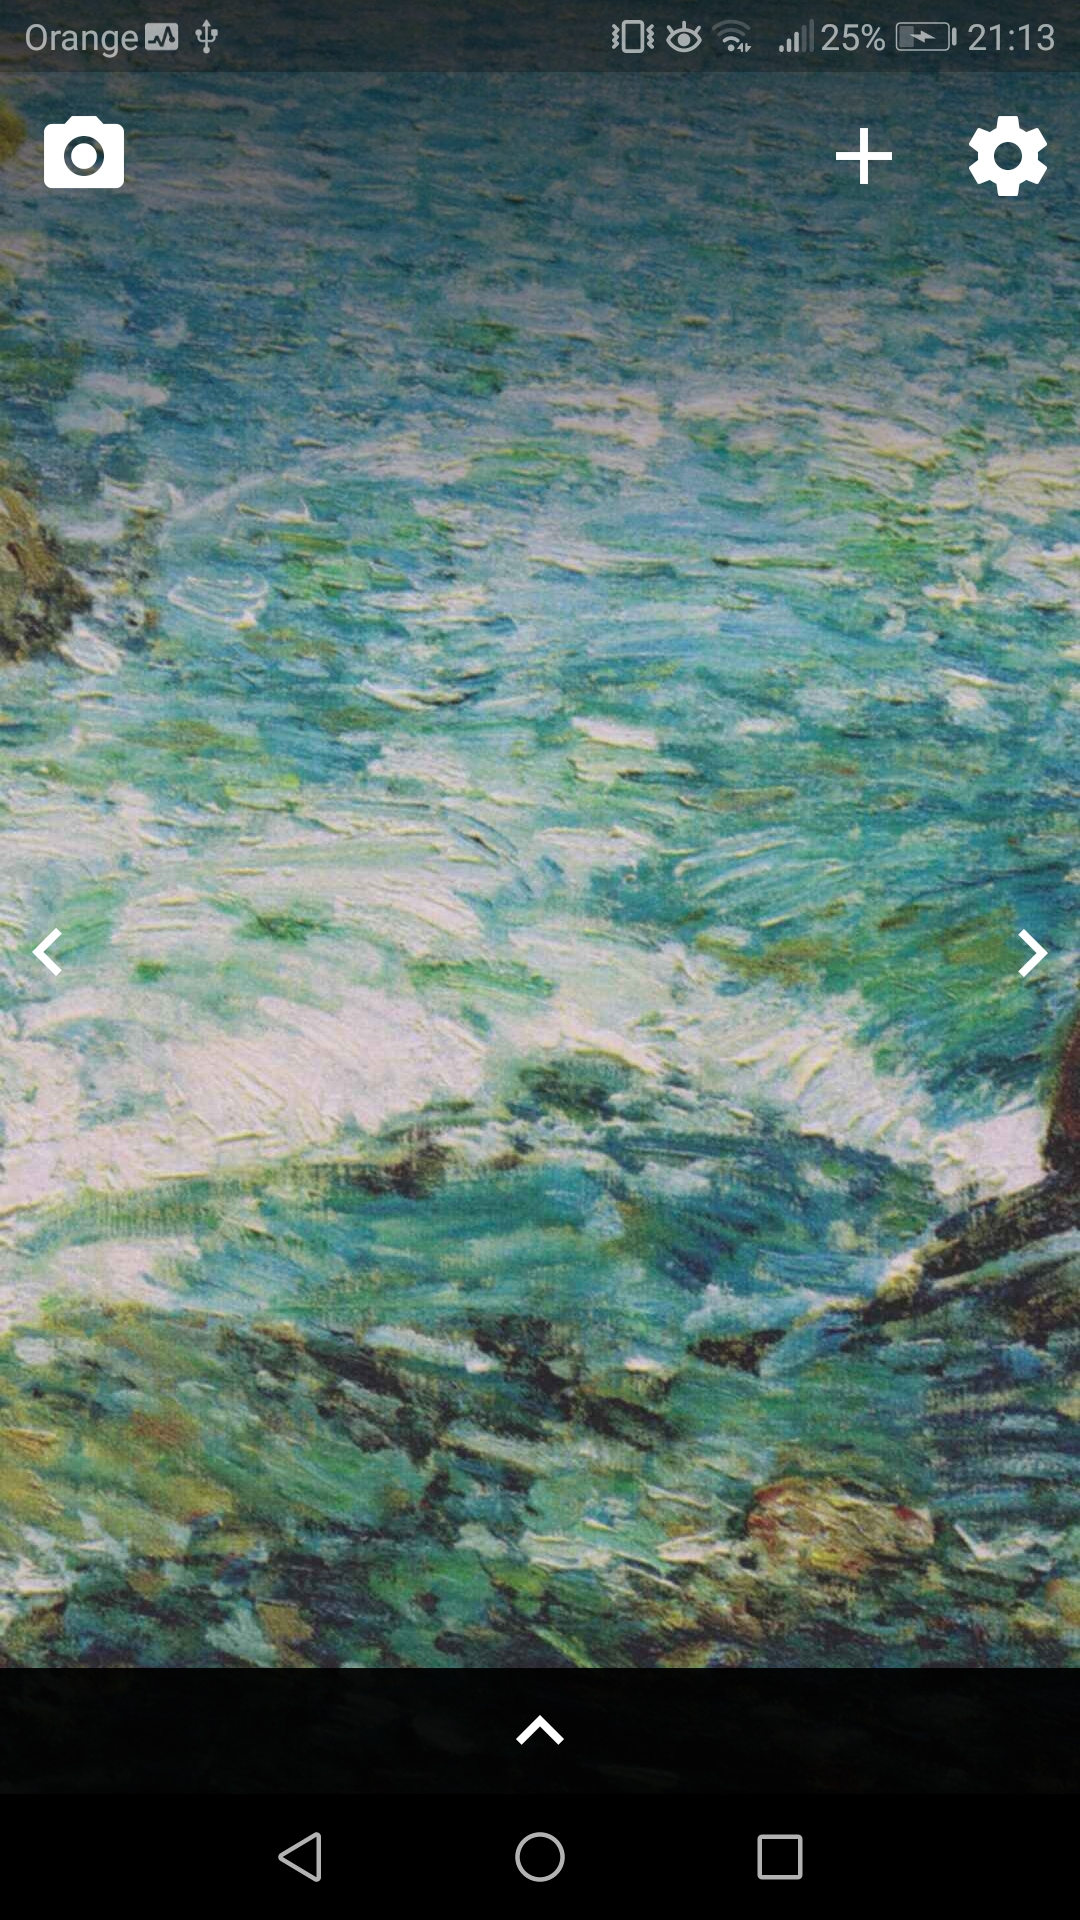
\includegraphics[width=\linewidth]{gallery_2.jpg}
        \caption{Folded gallery}\label{fig:gallery_folded}
    \endminipage\hfill
    \minipage{0.32\textwidth}
        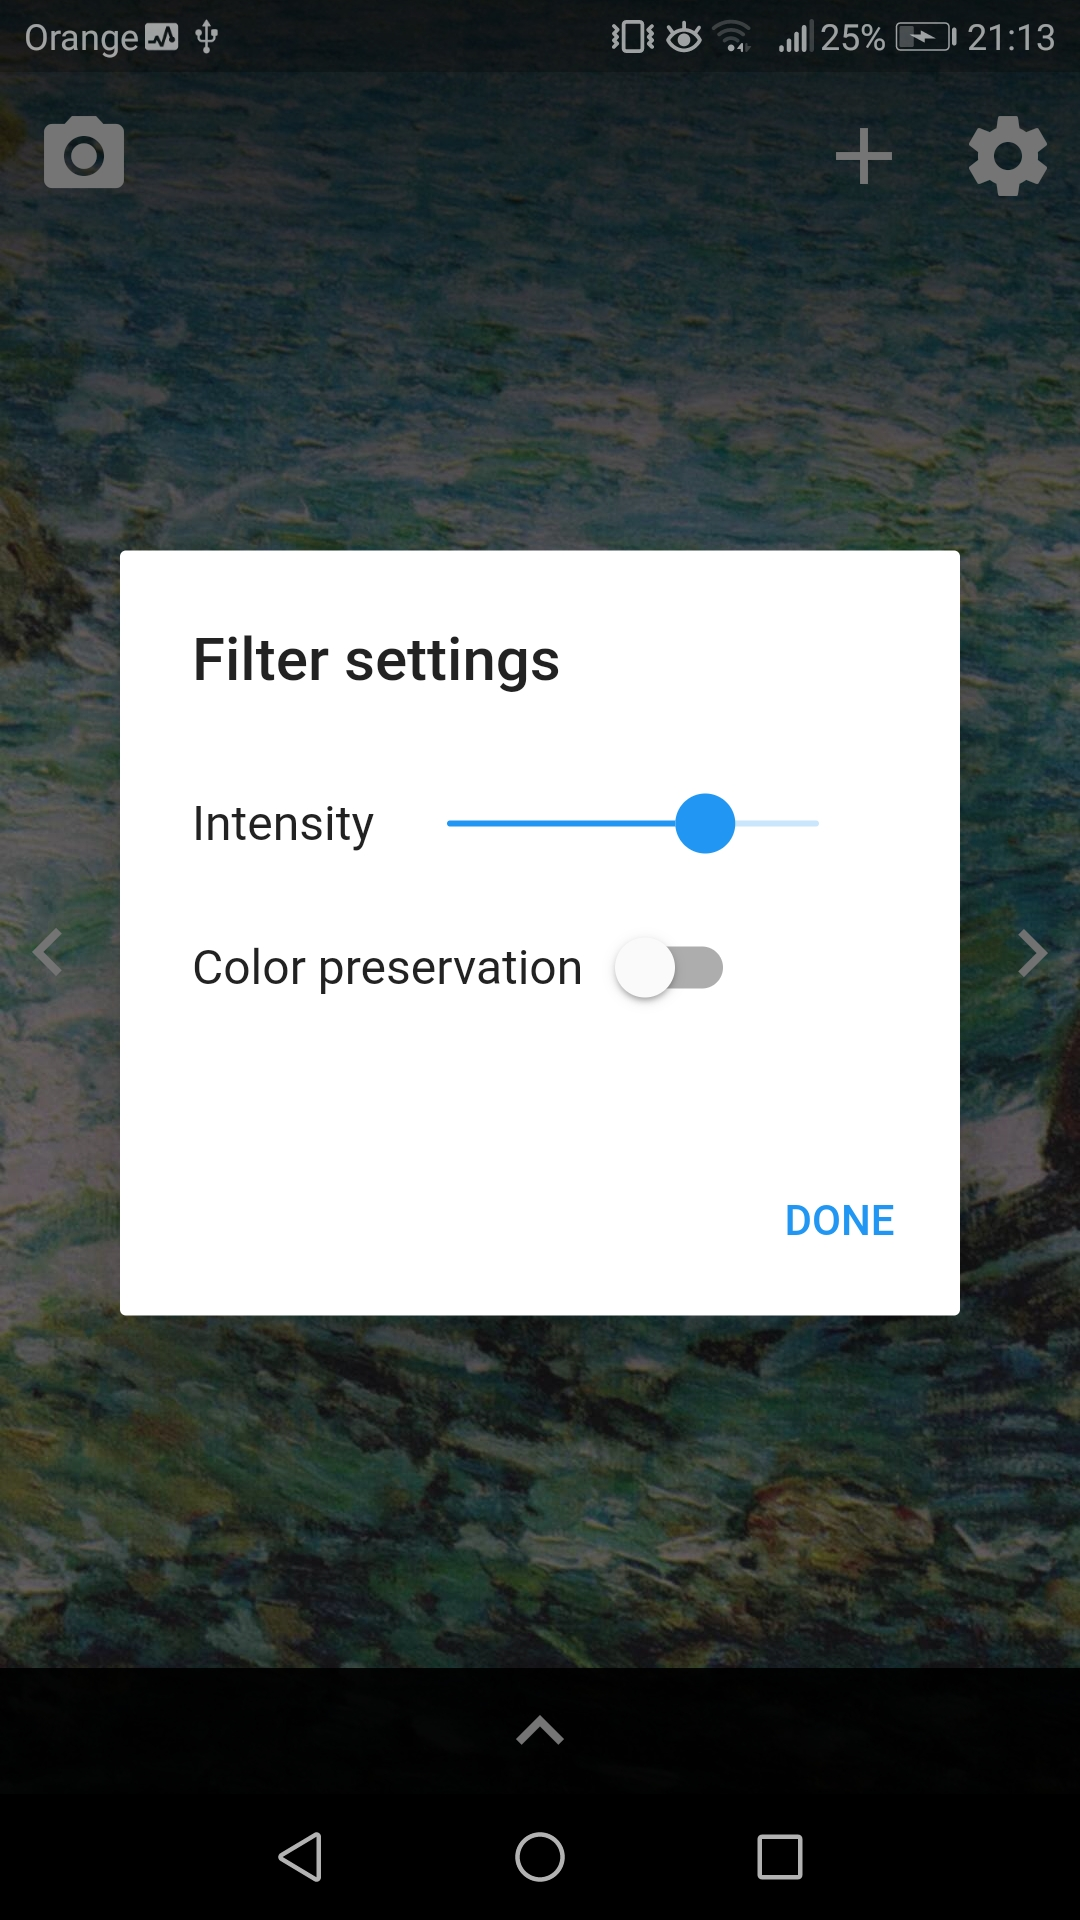
\includegraphics[width=\linewidth]{options.jpg}
        \caption{Settings}\label{fig:gallery_options}
    \endminipage\hfill
\end{figure}


\subsubsection{Style transfer screen}
When we finally pick our filter and settings we can start style transfer.
Whole screen screen is filled with transformed video.
If we don't like current filter or want to stop style transfer all we need to 
do is push \textit{X} button on the bottom of the screen 
and then we will go back to gallery.

\begin{figure}[H]
    \minipage{0.32\textwidth}
        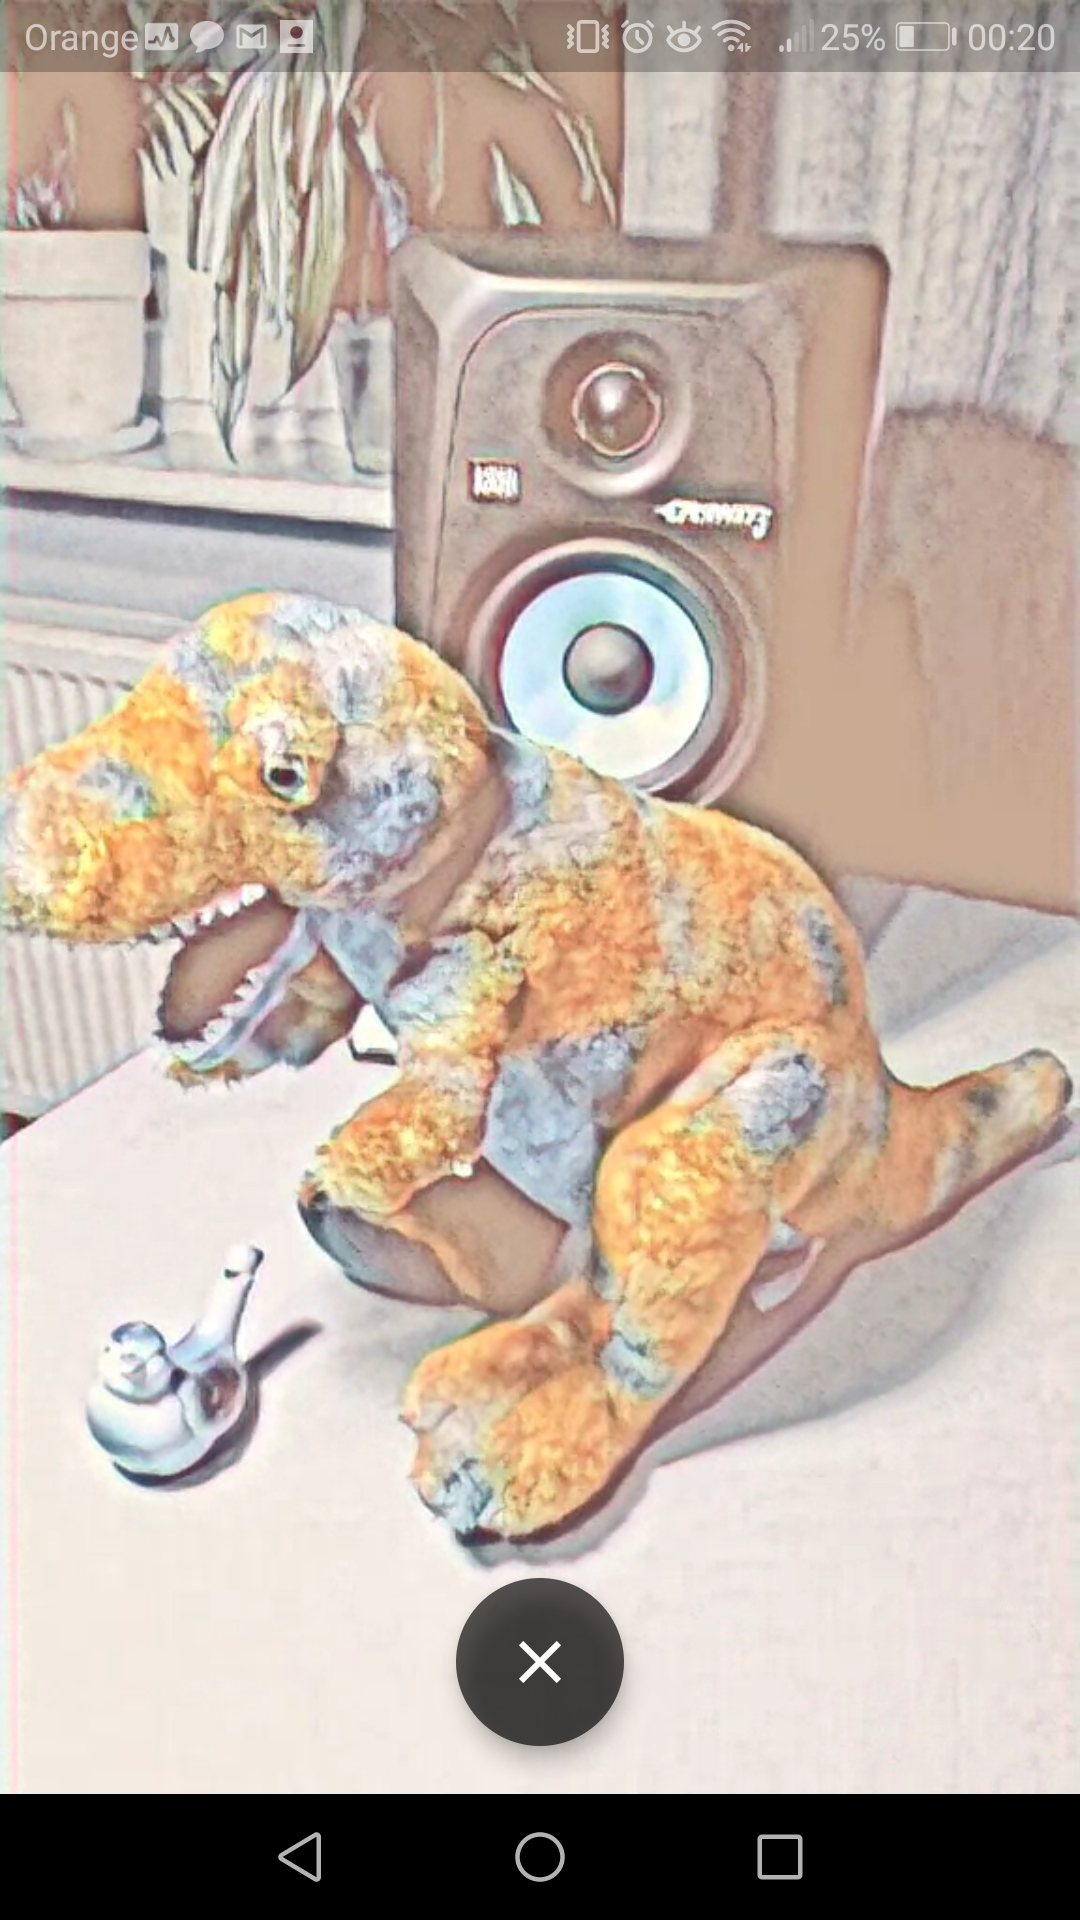
\includegraphics[width=\linewidth]{Images/dino4.jpg}
    \endminipage\hfill
    \minipage{0.32\textwidth}
        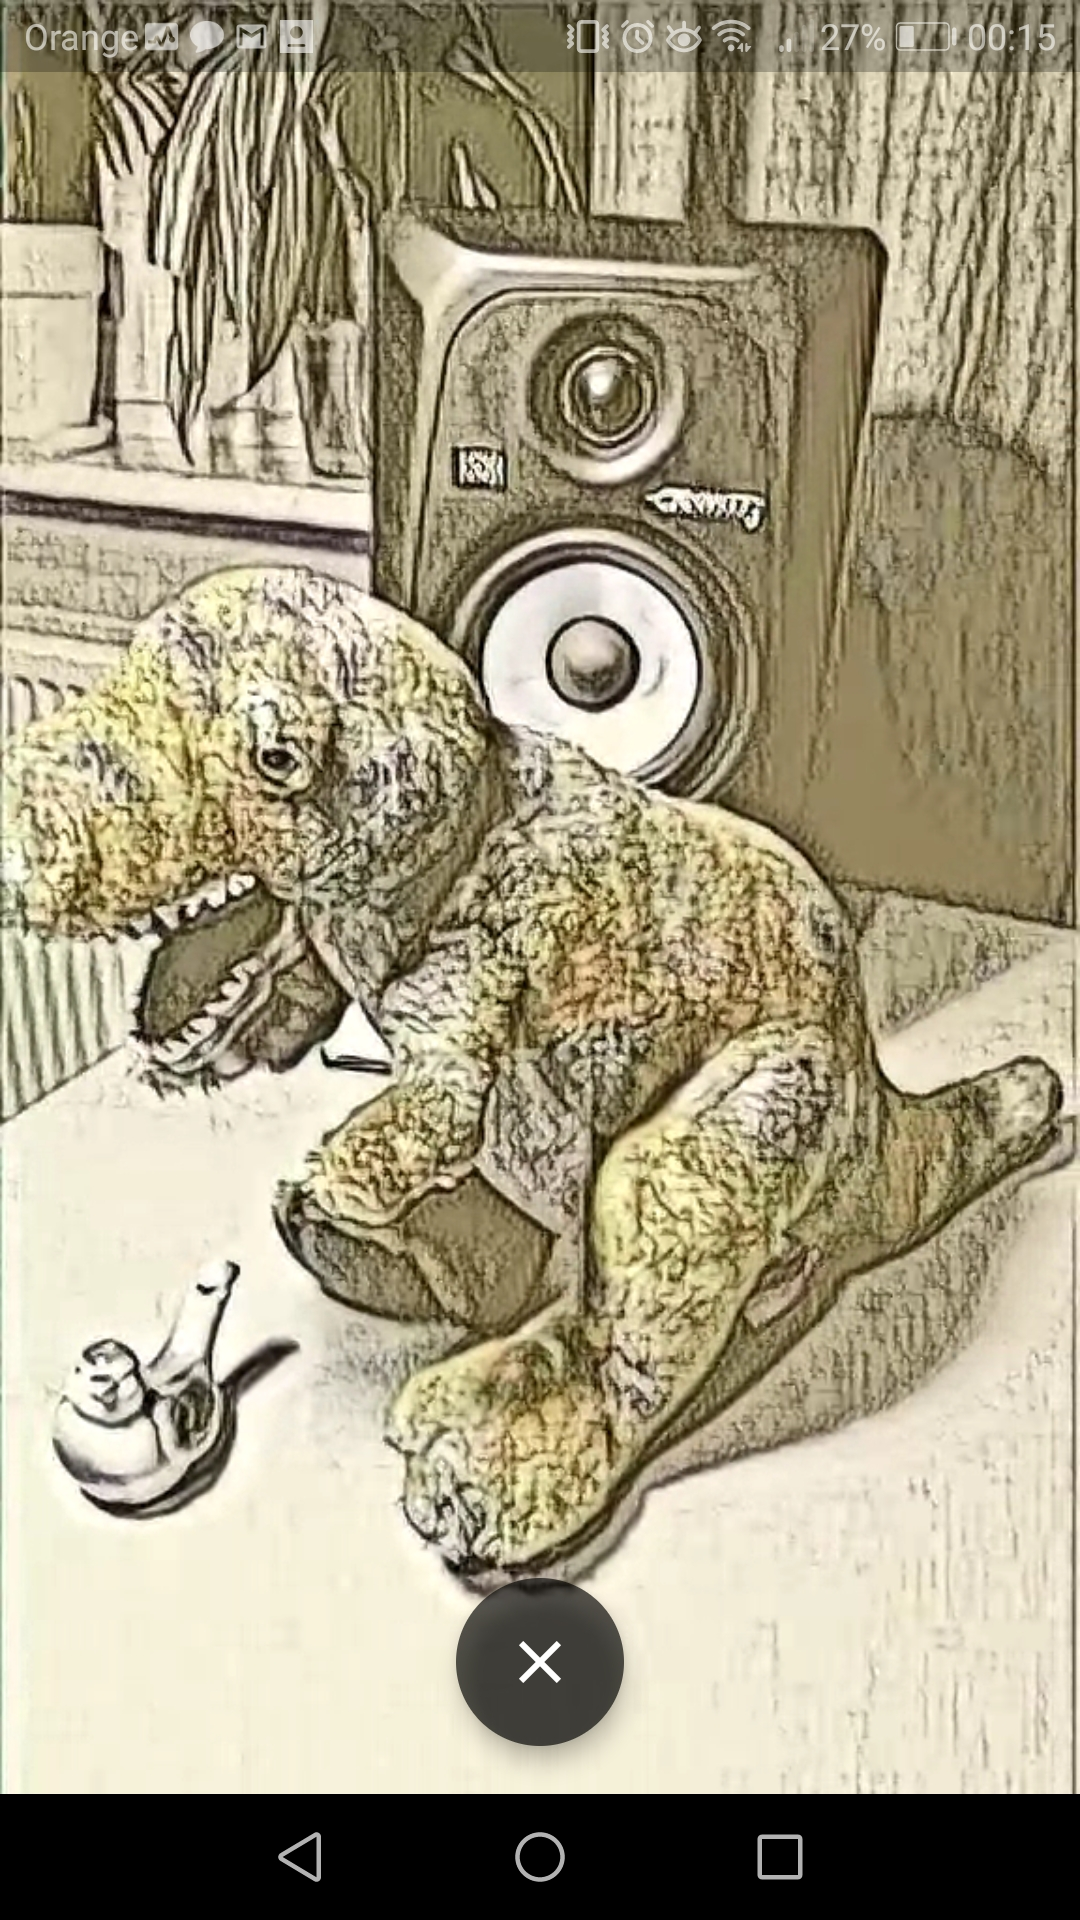
\includegraphics[width=\linewidth]{Chapters/dino2.jpg}
    \endminipage\hfill
    \minipage{0.32\textwidth}
        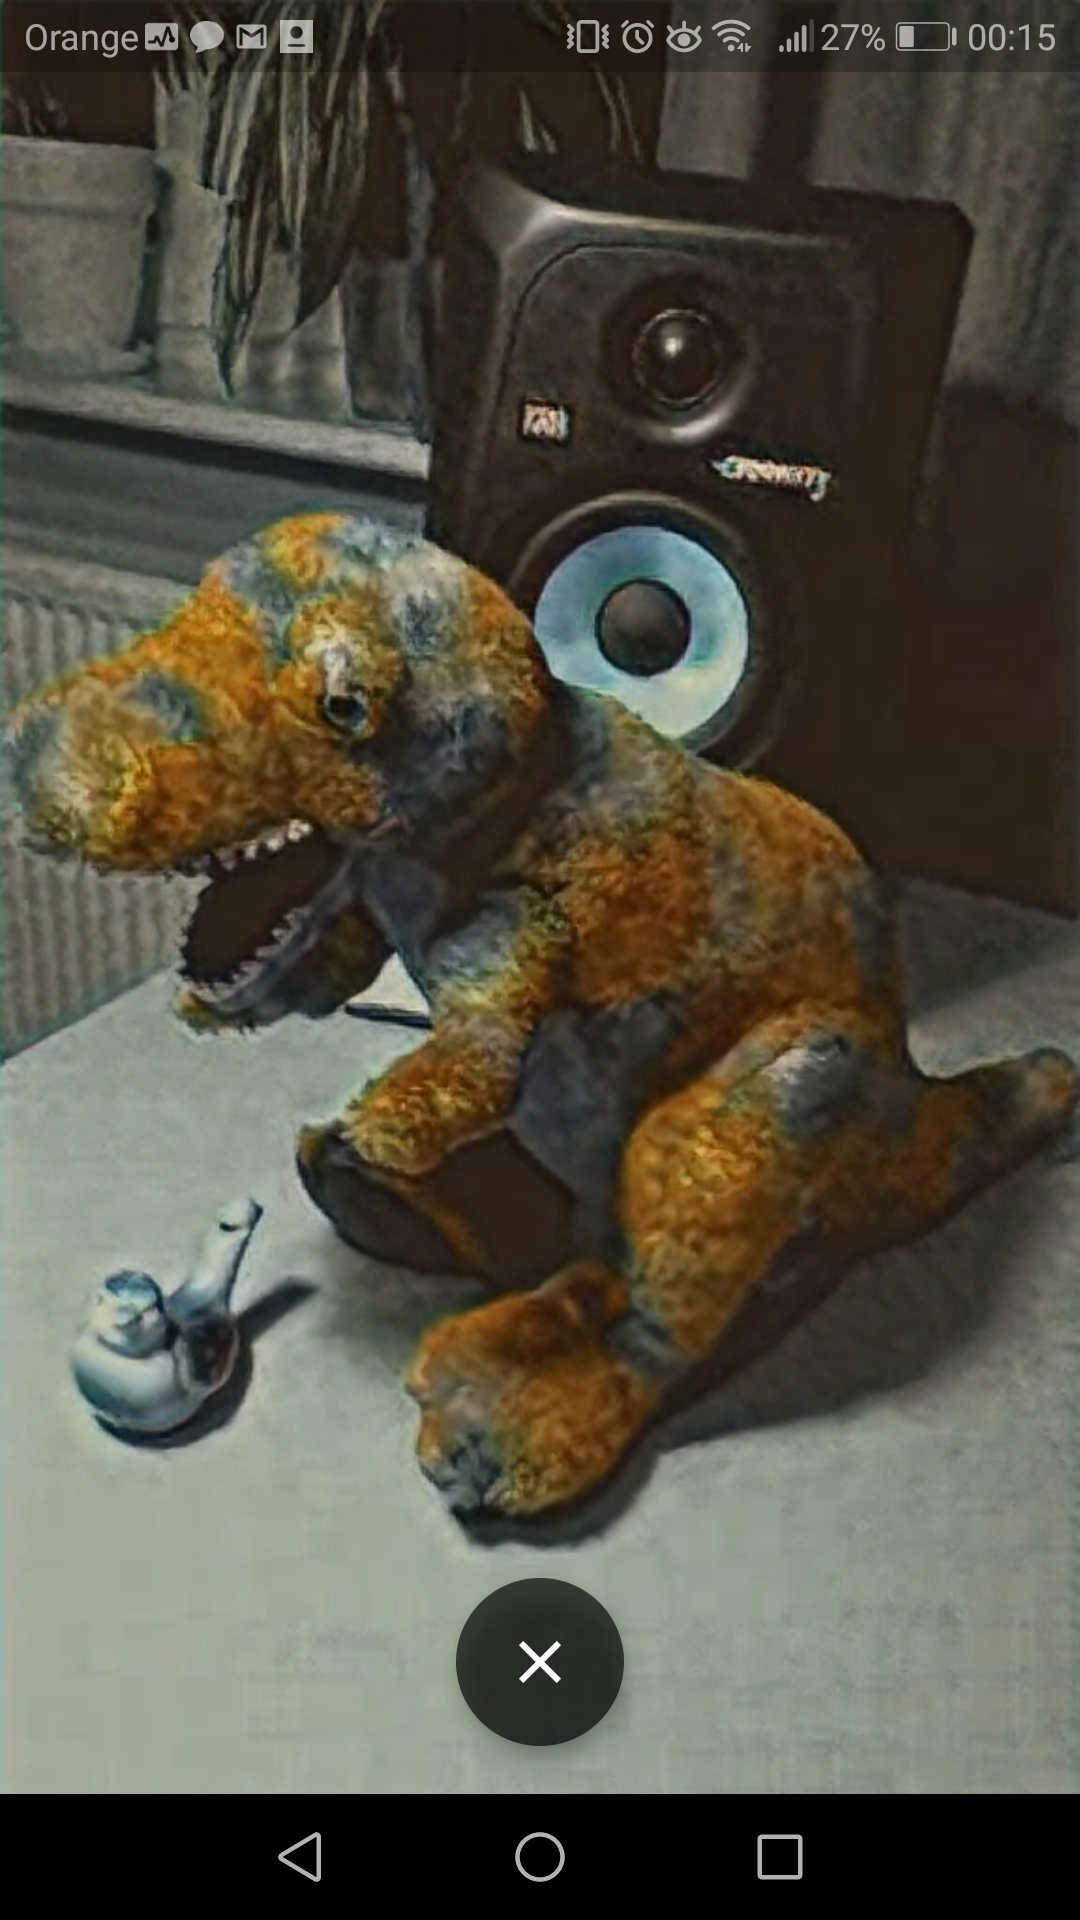
\includegraphics[width=\linewidth]{Chapters/dino3.jpg}
    \endminipage\hfill
    \caption{Style transfer with different filters}\label{fig:gallery_options}
\end{figure}


\subsubsection{\textit{Pick a filter} screen}
We anticipated that there might be a situation that the users will notice a ravishing 
scenery or a breathtaking view they can use it as a filter.
There is an opportunity to pick a photo quickly and than start style transfer immediately.
On the Figure \ref{fig:preview} we can see camera preview from back camera.
User can also switch to front camera by clicking \textit{switch camera}
icon in top right corner.
After we take picture we are redirected to screen presented on Figure 
\ref{fig:taken_photo} and then we can decide whether use picked photo as filter or not.
If we are satisfied with filter image we have to press \textit{Style it} button.
After that style transfer begins.


\begin{figure}[H]
    \centerline{
    \minipage{0.32\textwidth}
        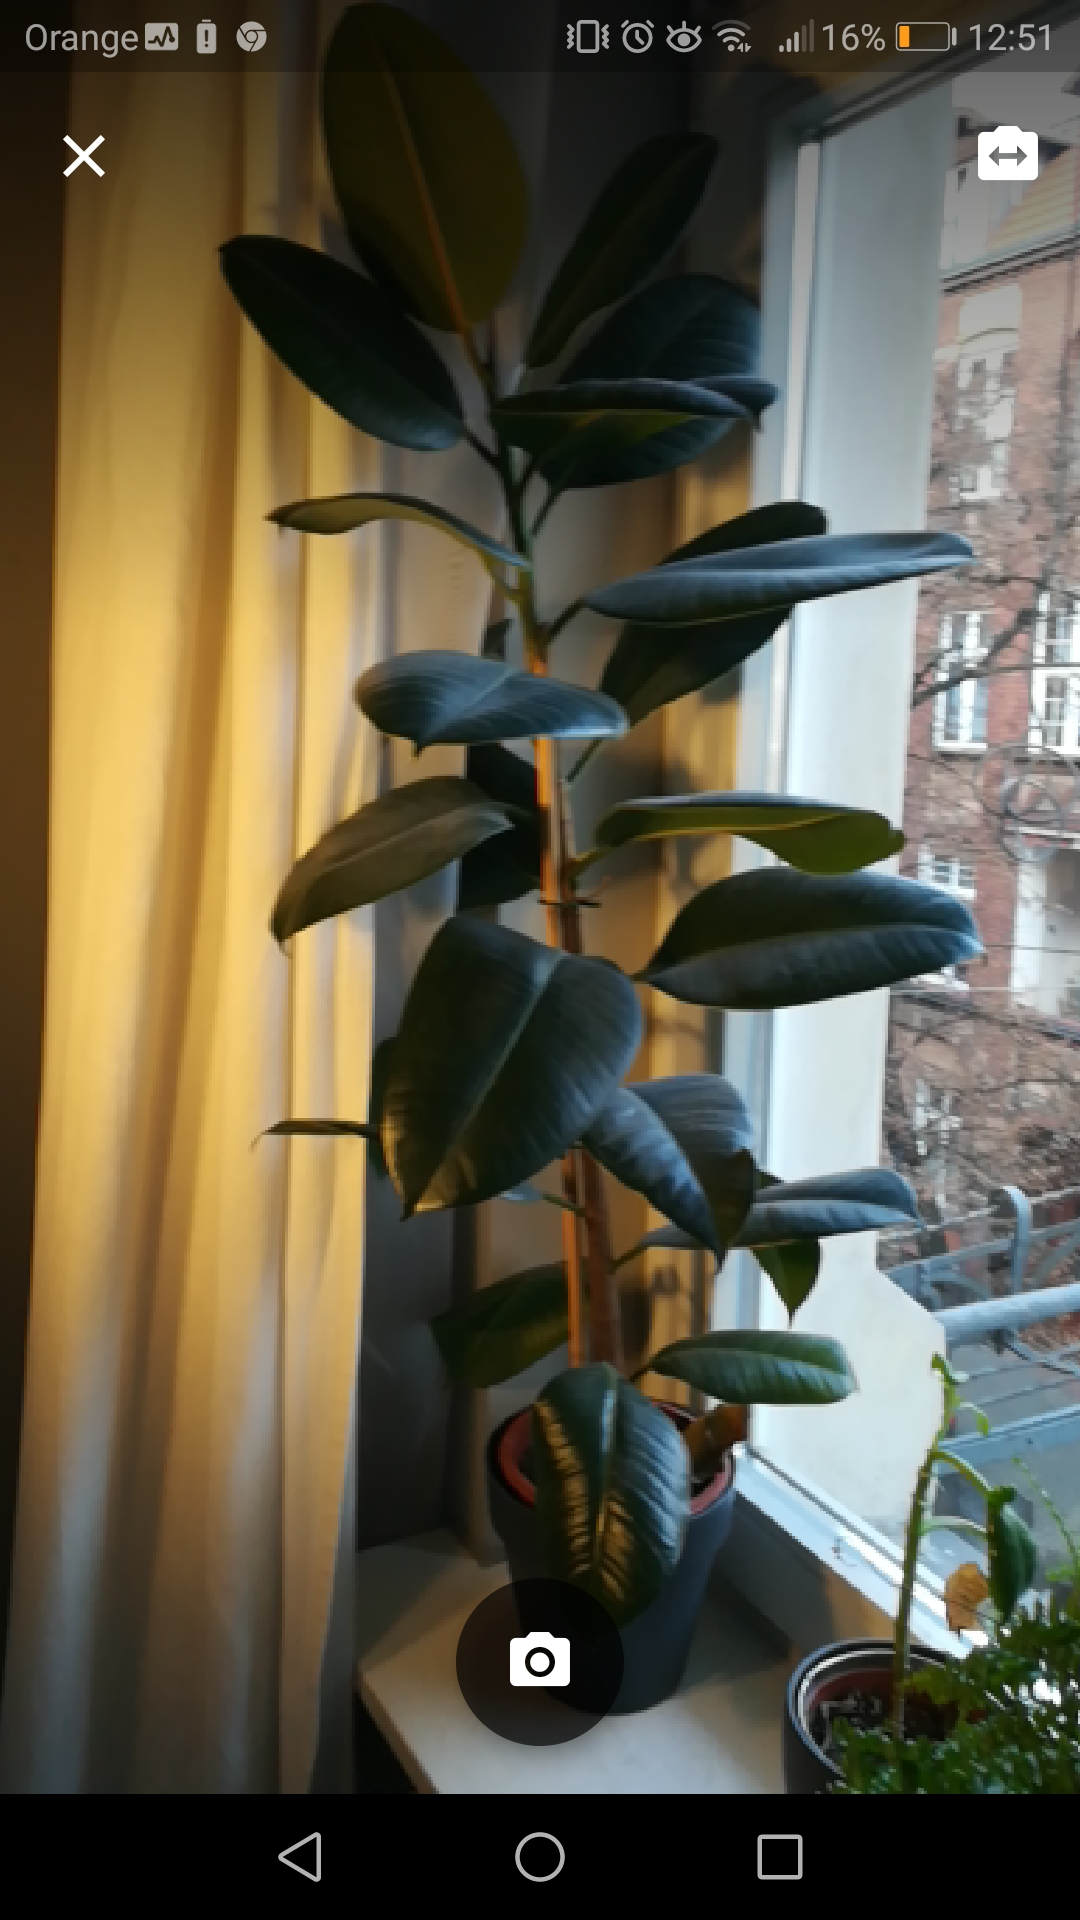
\includegraphics[width=\linewidth]{pick2.jpg}
        \caption{Camera preview}\label{fig:preview}
    \endminipage\hspace{0.01\textwidth}
    \minipage{0.32\textwidth}
        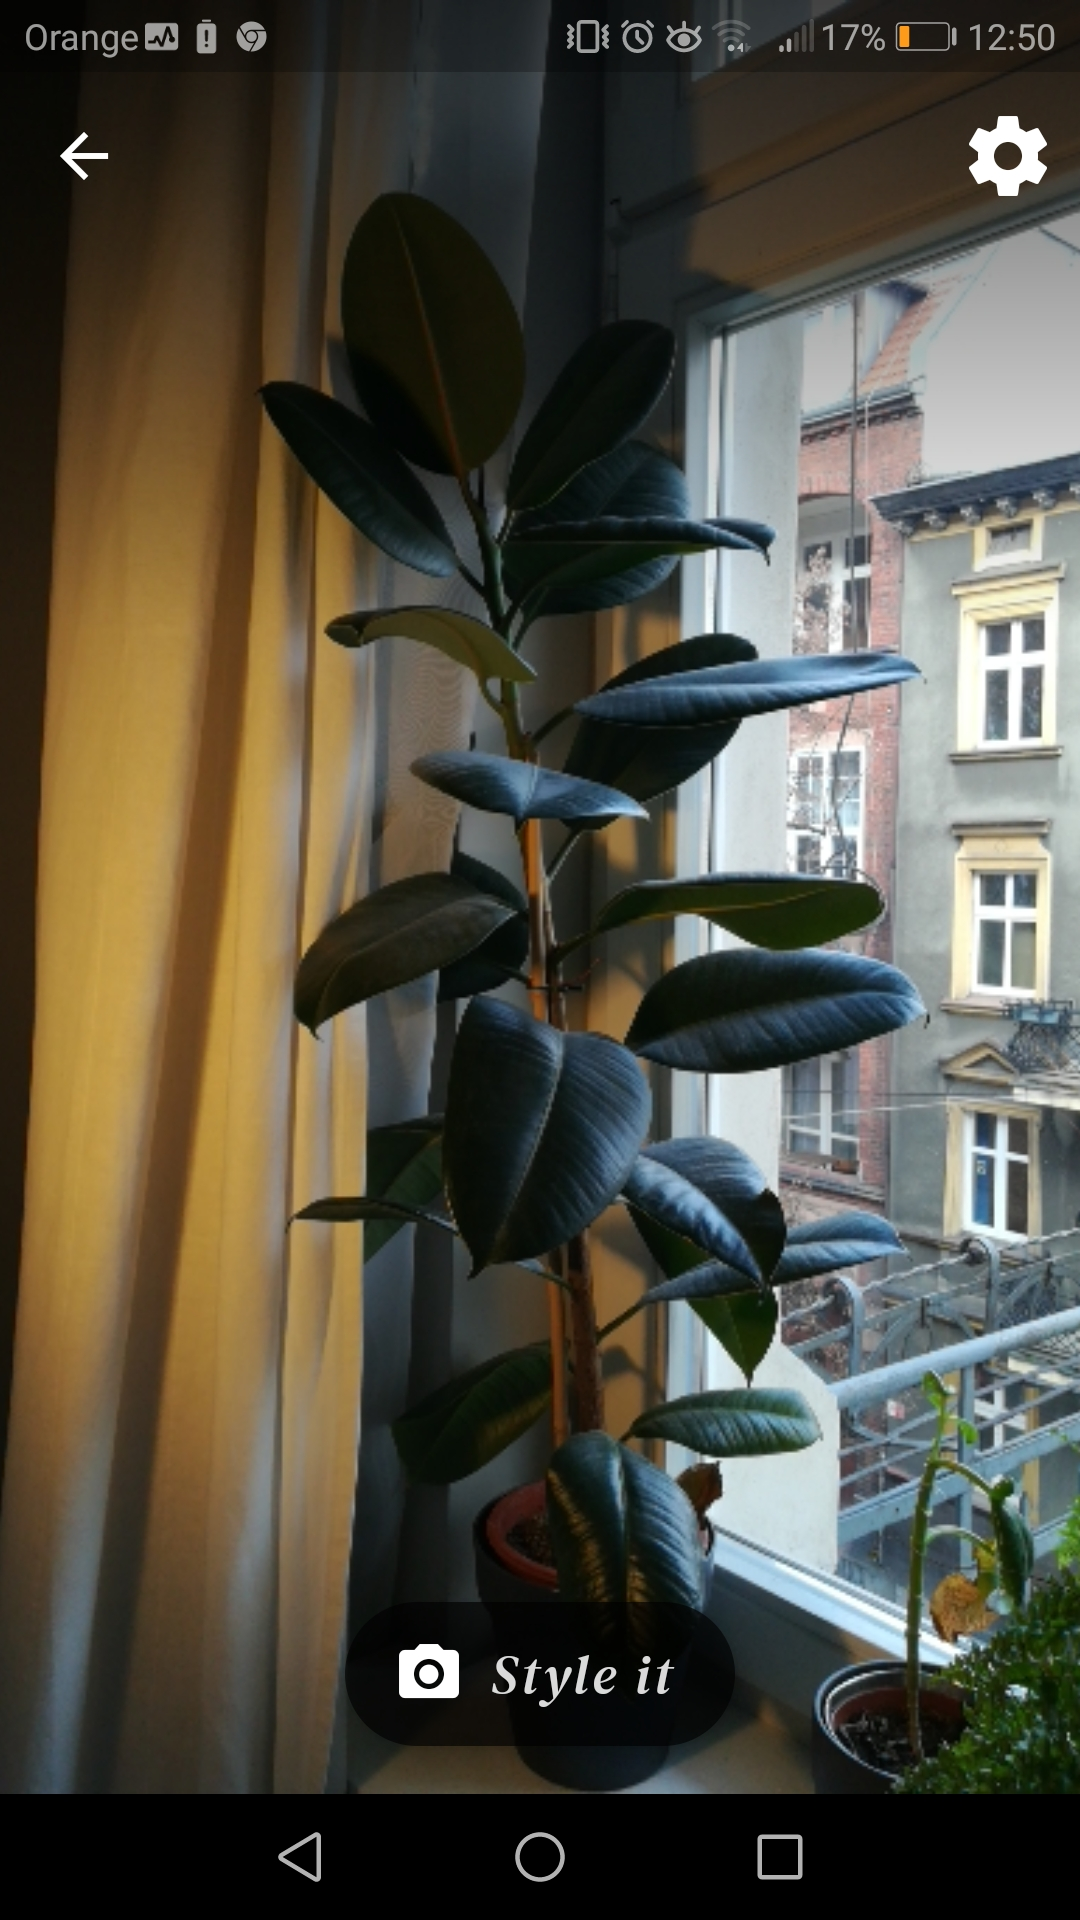
\includegraphics[width=\linewidth]{pick1.jpg}
        \caption{Taken photo}\label{fig:taken_photo}
    \endminipage}
\end{figure}



























\end{document}
